\documentclass[8pt,apectratio=169]{beamer}

\usetheme[progressbar=frametitle]{metropolis}
\usepackage{appendixnumberbeamer}
\usepackage[style=authoryear, backend=bibtex8, natbib=true, maxcitenames=2]{biblatex}

\usepackage[utf8]{inputenc} % utf8x  defines more symbols, but may cause compatible problems
\usepackage{lmodern,textcomp} % Latin Modern fonts, contains €

\usepackage{graphicx}
\usepackage{import}

\usepackage{booktabs}
\usepackage[scale=2]{ccicons}

\usepackage{pgfplots}
\usepgfplotslibrary{dateplot}

\usepackage{xspace}
\newcommand{\themename}{\textbf{\textsc{metropolis}}\xspace}

% Math
\usepackage{amsmath}
\usepackage{bm} % bold symbol in math mode

% Optional packages
\usepackage{multicol}
\usepackage{hyperref}
\usepackage[super,negative]{nth} % allows writing 1st, 2nd, 3rd with superscript
%\usepackage{ulem} % use the "sout" tag to "strikethrough" text


% Select what to do with command \comment:
  % \newcommand{\comment}[1]{}  %comments not shown
   \newcommand{\comment}[1]{\par {\bfseries \color{blue} #1 \par}} %comment showed

% Select what to do with todonotes: i.e. \todo{}, \todo[inline]{}
  % \usepackage[disable]{todonotes} % notes not shown
  \usepackage[draft]{todonotes}   % notes shown

  %\numberwithin{equation}{section}


\addbibresource{bib_energy}

\titlegraphic{\hfill 
\includegraphics[width=0.15 \textwidth]{graphics/logo}}
\title{Heterogeneity in demand responses to electricity spot prices}
\date{May 8 2019} % \today
\author{Thor Donsby Noe
        \and Cathrine Falbe Pedersen    }
\institute{\normalsize Department of Economics,
            University of Copenhagen \\
            \small Seminar in Energy Economics w. Frederik Roose Øvlisen}
%\institute{Department of Economics, University of Copenhagen}

    % \definecolor{BlueTOL}{HTML}{222255}
    \definecolor{BrownTOL}{HTML}{666633}
    \definecolor{GreenTOL}{HTML}{225522}
    % \setbeamercolor{normal text}{fg=BlueTOL,bg=white}
    \setbeamercolor{alerted text}{fg=BrownTOL}
    \setbeamercolor{example text}{fg=GreenTOL}

    \setbeamercolor{block title alerted}{use=alerted text,
        fg=alerted text.fg,
        bg=}
    \setbeamercolor{block body alerted}{use={block title alerted, alerted text},
        fg=alerted text.fg,
        bg=}
    \setbeamercolor{block title example}{use=example text,
        fg=example text.fg,
        bg=}
    \setbeamercolor{block body example}{use={block title example, example text},
        fg=example text.fg,
        bg=}

    \setbeamercolor{block title alerted}{use=alerted text,
        fg=alerted text.fg,
        bg=alerted text.bg!80!alerted text.fg}
    \setbeamercolor{block body alerted}{use={block title alerted, alerted text},
        fg=alerted text.fg,
        bg=block title alerted.bg!50!alerted text.bg}
    \setbeamercolor{block title example}{use=example text,
        fg=example text.fg,
        bg=example text.bg!80!example text.fg}
    \setbeamercolor{block body example}{use={block title example, example text},
        fg=example text.fg,
        bg=block title example.bg!50!example text.bg}


\begin{document}
\setbeamercolor{background canvas}{bg=white}
\maketitle


% ------------------------------------------------------------------------------
% ------ FRAME -----------------------------------------------------------------
% ------------------------------------------------------------------------------
\section{Outline}
\begin{frame}{Outline}
\tableofcontents
\end{frame}


\section{Introduction}

\begin{frame}{Motivation}
\begin{multicols}{2}
\begin{itemize}
    \item Change towards more electricity production by renewable sources
    \item Only sustainable if demand can be directed to when production is ongoing
    \item[$\rightarrow$] How does demand respond to price changes in electricity?
\end{itemize}
\vfill\null\columnbreak
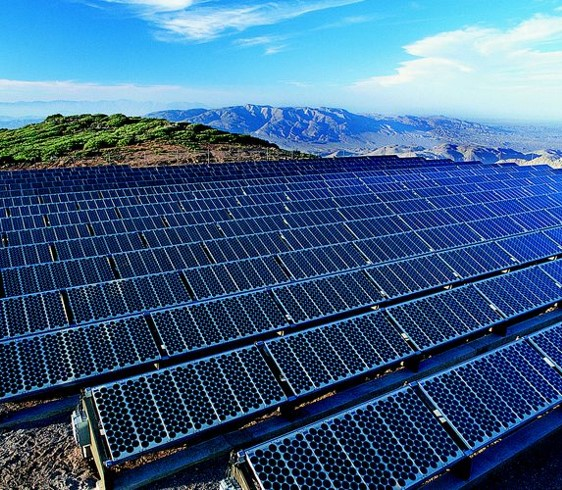
\includegraphics[width=0.5 \textwidth]{graphics/solar_panels}
\end{multicols}
\end{frame}


\section{Background}

\begin{frame}{Existing literature}
\begin{multicols}{2}
Modest elasticities and limited data
\begin{itemize}
    \item \citet{lijesen2007real} finds a peak elasticity of -0.0043 for hour-by-hour total Dutch consumption, \citet{wolak2001impact} find peak elasticities of -0.05 on half-hourly consumption for 5 British industries.
    \item In 36 non-time-of-day studies estimates range between -0.004 to -2.01 with median -0.81 in the short run (meta analysis)
    \item Experiments with time-of-use tariffs
\end{itemize}
%\vfill\null
\columnbreak
Heterogeneity
\begin{itemize}
    \item Across industries (UK)
    \item Under extreme weather (AUS)
    \item Under extreme prices (UKR)
\end{itemize}
Instrumenting for electricity spot price
\begin{itemize}
    \item Lagged prices at cost of dynamic bias (using GMM estimation)
    \item Use wind speed as instrument (DEU)
\end{itemize}
\end{multicols}
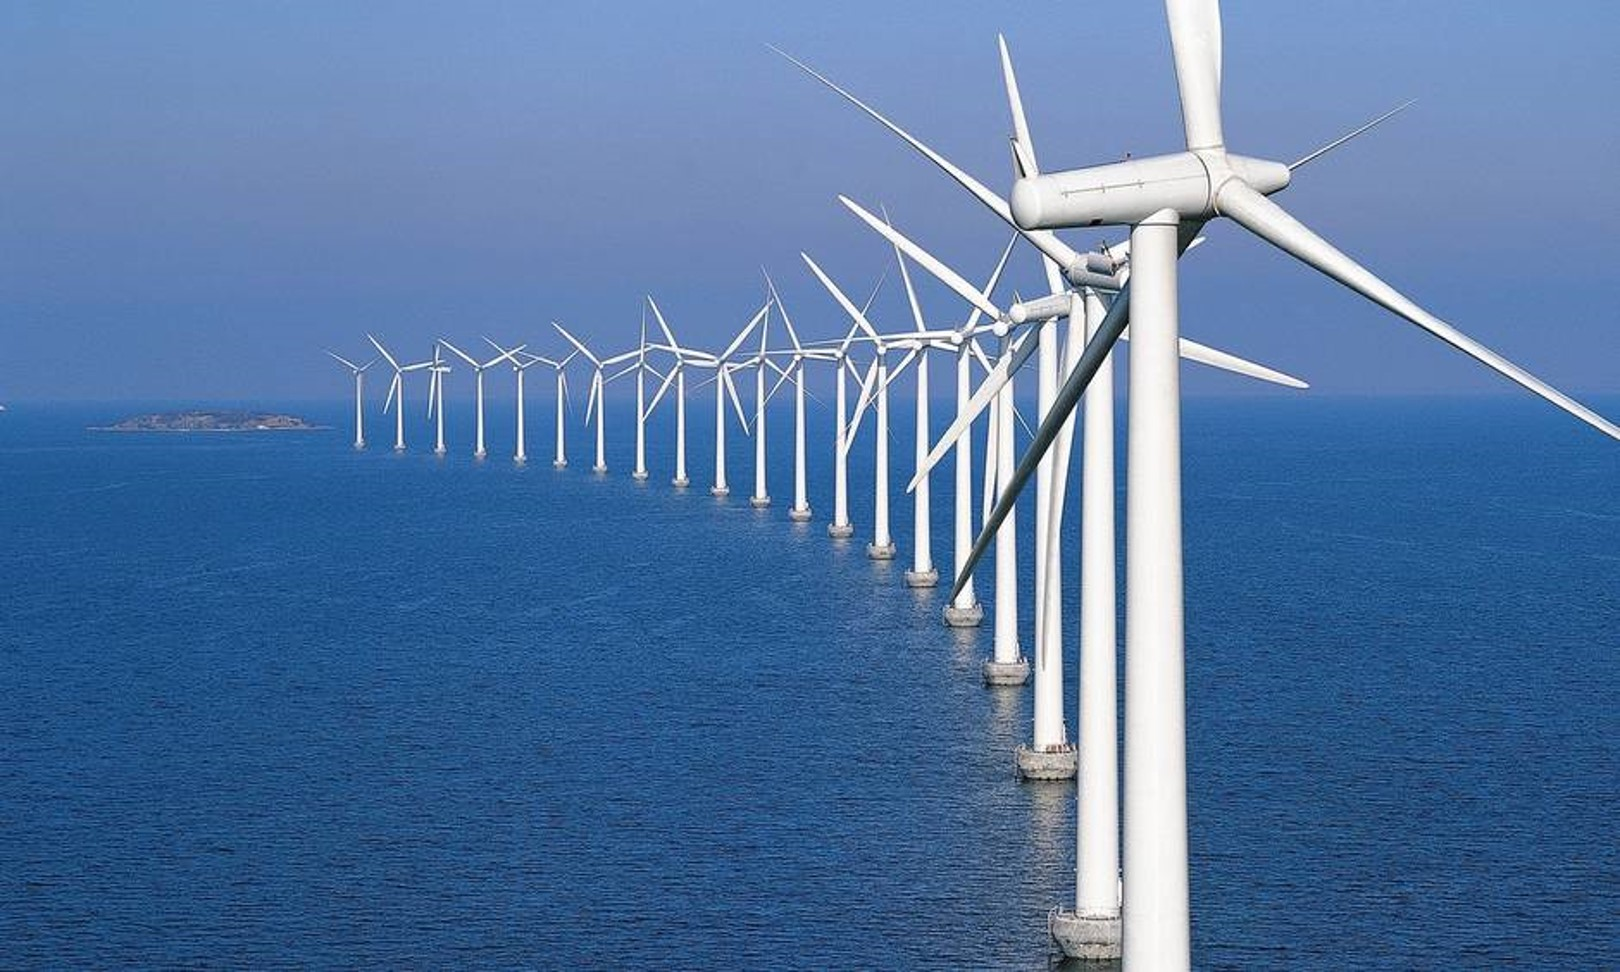
\includegraphics[width=1 \textwidth]{graphics/wind_mills}
\end{frame}


\begin{frame}{Our contribution}
\begin{multicols}{2}
Hour-by-hour data
\begin{itemize}
    \item For both consumption and prices
\end{itemize}
Separate data for:
\begin{enumerate}
    \item Wholesale consumption
    \item Retail consumption\\
          (full population, not a survey)
\end{enumerate}
A degree of regional disaggregation
\begin{itemize}
    \item 52 different grid companies
\end{itemize}
New data (2016-2018)
\begin{itemize}
    \item Ever increasing share of renewables calls for flexibility
    \item First look at time-of-use tariff introduced December 2017
\end{itemize}
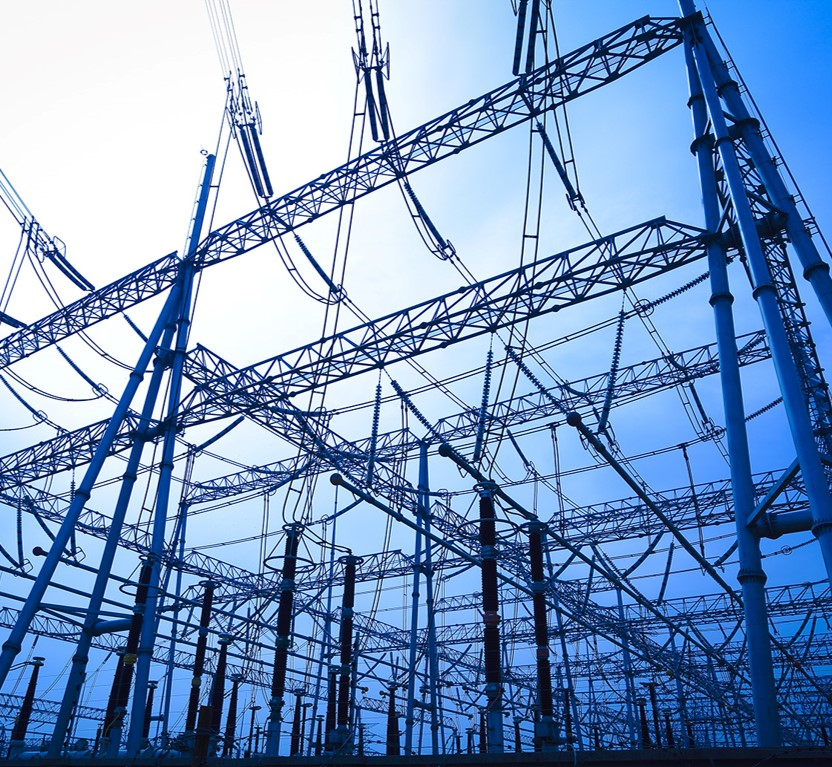
\includegraphics[width=0.6 \textwidth]{graphics/transformer}
\end{multicols}
\end{frame}


\section{Economics theory}
\begin{frame}{Price formation in the electricity market}
Electricity different from other goods: Essentially impossible to store
\begin{itemize}
    \item[$\rightarrow$] Demand $\leq$ Supply at any given point in time
    \item Surplus is costly and inefficient
\end{itemize}
Organisation of market:
\begin{enumerate}
    \item Long term contracts and forward market
    \item Day-ahead market (80 per cent of volume traded)
    \item Intra-day market
    \item Balancing market
\end{enumerate}
Production in merit order after marginal price
\begin{itemize}
    \item E.g. wind power $>$ hydro $>$ coal $>$ gas
    \item Thus, wind power prognosis $\rightarrow$ decrease in spot price
\end{itemize}
\end{frame}


\begin{frame}{Demand for electricity}
Electricity demand is shaped by the demand for the use of other appliances that require electricity to function
\begin{itemize}
    \item[$\rightarrow$] Even less information on costs is available to the consumer which makes responding difficult
    \item Calculating the price of using an appliance requires knowledge of both electricity prices and how much each device uses
    \item Implies that many consumers rely on behavioral rules when deciding on electricity consumption
\end{itemize}
Important distinction
\begin{itemize}
    \item Wholesale consumers (large and medium-sized firms)
    \item Retail consumers (households and small firms)
\end{itemize}
\end{frame}


\section{Data}

\begin{frame}{Data and variables}
Consumption for 2016-2018:
\begin{itemize}
    \item Grid-level hourly consumption and number of electricity-meters, split by
    \begin{enumerate}
        \normalsize
        \item hourly-settled (wholesale)
        \item flex-settled from December 2017 (retail)
        \item residual consumption (retail)
    \end{enumerate}
    \item Scraped from \href{https://www.energidataservice.dk/en/}{Energinet} via SQL statements
\end{itemize}
Prices and wind power
\begin{itemize}
    \item Spot-price in the day-ahead-market
    \item Wind power prognosis
    \item Downloaded from \href{https://www.nordpoolgroup.com/historical-market-data/}{Nord Pool}
\end{itemize}
Weather variables
\begin{itemize}
    \item Temperature (scraped from \href{https://www.dmi.dk/vejrarkiv/}{DMI})
    \item Daytime variable using sunset and sunrise (scraped from \href{https://soltider.dk/}{soltider.dk})
    \item Collected for the two biggest municipalities, Aarhus and Copenhagen
    \begin{itemize}
        \normalsize
        \item[$\rightarrow$] Extrapolated to all grids of price region DK1 and DK2 respectively
    \end{itemize}
\end{itemize}
Time variables
\begin{itemize}
    \item Time trend
    \item Calendar dummies and interactions with hour-of-day
    \item Sample split by business days and non-business days (holidays and weekends)
\end{itemize}
\end{frame}

\begin{frame}
\begin{figure}[H]
  \centering
  \caption{Mean electricity consumption by hour}
    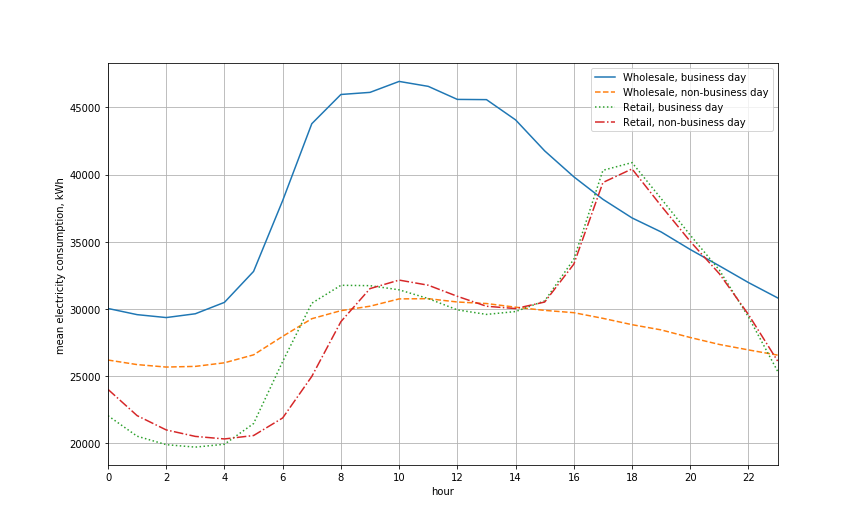
\includegraphics[width=1. \textwidth]{graphics/hours}
  \label{fig:cons_hour}
\end{figure}
\end{frame}


\section{Empirical strategy}

\begin{frame}{Specifications}
  \textbf{Baseline model} for log electricity consumption, $\ln e_{it}$, in grid $i$ at time $t$ (date by hour)
  \begin{equation}
   \begin{split}
    \ln e_{it}=& \underbrace{\varepsilon \hat{\ln p_{rt}}}_\text{Spot price in price region}+\underbrace{\delta\ln n_{im}}_\text{Number of meters by \nth{1} of the month}+\underbrace{\bm{w}^{'}_{rt}\lambda}_\text{Weather}+\underbrace{\gamma\ days}_\text{Time trend}\\
    &+\underbrace{\eta_{year}+\eta_{week}}_\text{Year and week dummies}+\underbrace{\eta_{month}\cdot\eta_{hour}+\eta_{day}\cdot\eta_{hour}}_\text{Consumption pattern by month and weekday}+\underbrace{c_i}_\text{Grid effect}+u_{it}
   \end{split}
   \label{eq:baseline}
  \end{equation}
  \textbf{Effect of time-of-use-tariff} in grid company Radius
  \begin{itemize}
      \item Since December 2017: Time-of-use tariff for the hours 17-19 during Winter
      \item Estimated using baseline specification (\ref{eq:baseline}) but only for Radius and hours 17-19
      \begin{itemize}
          \normalsize
          \item Without the grid-specific time-invariant constant term $c_i$
          \item But including a term for the effect of the TOU tariff:
      \end{itemize}
      \begin{align}
        \alpha\frac{nf_{month}}{nr_{month}}\tau_{year,month}
        \label{eq:tout}
      \end{align}
      \begin{itemize}
        \normalsize
        \item $\frac{nf_{month}}{nr_{month}}$ is the share of retail meters constituted by flex-settled meters
        \item $\tau$ is a dummy for the months October-March after December 2017
      \end{itemize}
  \end{itemize}
\end{frame}

\begin{frame}{Random Effects estimation (RE)}
Different candidates for panel data estimation
\begin{itemize}
    \item Least Squares Dummy Variables estimation (LSDV)
    \begin{itemize}
        \item Unobserved heterogeneity, $c_i>0$, leads to serial correlation
    \end{itemize}
    \item Fixed Difference estimation (FD)
    \begin{itemize}
        \item Strict exogeneity assumption, $cov(u_{it},\bm{x}_{it})=0$, is violated by hourly-patterns
    \end{itemize}
    \item Fixed Effects estimation (FE)
    \begin{itemize}
        \item Time-demeaned, too extreme
    \end{itemize}
    \item Dynamic Panel Estimation using Generalized Methods of Moments (GMM)
    \begin{itemize}
        \item Only necessary if including lagged prices as instruments
    \end{itemize}
\end{itemize}
We choose the \textbf{Random Effects estimator (RE)} for wholesale consumption
\begin{itemize}
    \item Critical assumption for RE: No endogeneity, i.e. $cov(c_i,\bm{x}_{it})=0$.
    \item Hausman test: $\hat{\beta}^{*}_{RE}=\hat{\beta}^{*}_{FE}\rightarrow$ no endogeneity $\rightarrow$ both RE and FE are consistent, but RE is more efficient.
\end{itemize}
Estimate RE estimation using \textbf{feasible Generalized Least Squares (fGLS)}
\begin{itemize}
    \item[\nth{1} stage:] Estimate eq. (\ref{eq:baseline}) using LSDV estimation $\rightarrow$ store $\hat{\lambda}=1-\left(\frac{\sigma^2_u}{\sigma^2_u+T\sigma^2_\alpha}\right)^\frac{1}{2}$
    \item[\nth{2} stage:] LSDV using $\hat{\lambda}$ to estimate the quasi-time demeaned system of the form: $y_{it}-\hat{\lambda}\bar{y_i}=\beta_0(1-\hat{\lambda})+\beta_1(\bm{x}_{it}-\hat{\lambda}\bar{\bm{x}_i})+c_i(1-\hat{\lambda})+u_{it}-\hat{\lambda}u_{it}$.
\end{itemize}
\end{frame}

\begin{frame}{Instrumenting for prices}
Endogeneity problem
\begin{itemize}
    \item Price and demand affects each other simultaneously
    \item Wind power prognosis ($wpp$) is used as a proxy for predicted wind strength
    \begin{itemize}
        \item We expect different level and slope depending on being in Western Denmark ($DK1=1$)
        \item We expect an effect from $wpp$ in the other region as well due to electricity flows
    \end{itemize}
    \item However, $wpp$ is not completely exogenous but also considers spot prices.
\end{itemize}
Wholesale consumption with grid-specific time-invariant constant term, eq. (\ref{eq:baseline})
\begin{itemize}
    \item $\hat{\ln p_{rt}}=DK1\cdot wpp_{rt}+(1-DK1)\cdot wpp_{rt}+DK1\cdot wpp_{r-1,t}+(1-DK1)\cdot wpp_{r-1,t}+DK1$
    \item Estimated using the 3-stage Random Effects Instrumental Variables (REIV)
\end{itemize}
Retail consumption for the single grid Radius, including eq. (\ref{eq:tout})
\begin{itemize}
    \item $\hat{\ln p_{rt}}=wpp_{rt}+wpp_{r-1,t}$
    \item Estimated using 2SLS estimation
\end{itemize}
\end{frame}


\section{Results and discussion}

\begin{frame}{Elasticity for large and medium-sized firms}
\begin{table}[H]
  \vspace{-0.0cm}
  \centering
  \caption{log wholesale electricity consumption (REIV)}
  \footnotesize
    \begin{tabular}{lcccc}
      \toprule
        \begin{tabular}{lcccc}\toprule
                    &(1) Peak: 11-15   &(2) Off-peak: 00-04   &(3) Shoulder   &(4) Non-business day   \\
                    &        b/se   &        b/se   &        b/se   &        b/se   \\
\midrule
log spot price      &     -0.0484***&     -0.0266***&     -0.0333** &     -0.0189*  \\
                    &    (0.0163)   &    (0.0094)   &    (0.0149)   &    (0.0099)   \\
log wholesale meters&      0.1578***&      0.1422***&      0.1255***&      0.1424***\\
                    &    (0.0375)   &    (0.0399)   &    (0.0332)   &    (0.0375)   \\
Temperature         &     -0.0036***&     -0.0014** &     -0.0022***&     -0.0038***\\
                    &    (0.0008)   &    (0.0006)   &    (0.0004)   &    (0.0006)   \\
Temperature squared &      0.0002***&      0.0001***&      0.0001***&      0.0002***\\
                    &    (0.0000)   &    (0.0000)   &    (0.0000)   &    (0.0000)   \\
Daytime             &               &               &      0.0198***&      0.0966***\\
                    &               &               &    (0.0052)   &    (0.0085)   \\
Time variables      &         Yes   &         Yes   &         Yes   &         Yes   \\
\midrule
\(R^2\) within      &      0.3614   &      0.1576   &      0.5797   &      0.1414   \\
\(R^2\) between     &      0.9492   &      0.9140   &      0.9375   &      0.9250   \\
Number of groups    &          48   &          48   &          48   &          48   \\
Obs. per group      &       3,675   &       3,675   &      13,178   &       8,660   \\
\bottomrule\end{tabular}

    \end{tabular}
    \text{Cluster robust standard errors are in parentheses. * $p<0.10$, ** $p<0.05$, *** $p<0.01$.}
    \text{Log spot price is instrumented for by wind power prognosis for the same and the other region.}
  \label{tab:ws_preferred}
  \vspace{-0.0cm}
\end{table}
\end{frame}

\begin{frame}{Time-of-use tariff for households and small firms in Radius}
\begin{table}[H]
  \vspace{-0.0cm}
  \centering
  \caption{log retail electricity consumption in Radius, hours 17-19 (2SLS)}
  \footnotesize
    \begin{tabular}{lccc}
      \toprule
                            &(1) All days   &(2) Business days   &(3) Non-business days   \\
                    &        b/se   &        b/se   &        b/se   \\
\midrule
log spot price      &    -0.01597** &    -0.02624***&    -0.00515   \\
                    &   (0.00734)   &   (0.00803)   &   (0.01823)   \\
Time-of-use tariff  &    -0.01907** &    -0.01382*  &    -0.04444***\\
                    &   (0.00796)   &   (0.00800)   &   (0.01553)   \\
log household meters&    -0.92839   &    -1.31922   &    -0.29035   \\
                    &   (0.85359)   &   (0.92132)   &   (1.53637)   \\
Temperature         &    -0.00332***&    -0.00405***&    -0.00395***\\
                    &   (0.00058)   &   (0.00073)   &   (0.00133)   \\
Temperature squared &     0.00002   &     0.00004   &    -0.00000   \\
                    &   (0.00002)   &   (0.00003)   &   (0.00005)   \\
Daytime             &    -0.04708***&    -0.04502***&    -0.02614   \\
                    &   (0.01018)   &   (0.01084)   &   (0.01884)   \\
Time variables      &         Yes   &         Yes   &         Yes   \\
\midrule
Constant            &        26.6   &        32.2   &        13.3   \\
Observations        &       3,288   &       2,205   &       1,083   \\
\bottomrule

    \end{tabular}
    \text{Robust standard errors are in parentheses. * $p<0.10$, ** $p<0.05$, *** $p<0.01$.}
    \text{Log spot price is instrumented for by wind power prognosis for the same and the other region.}
  \label{tab:hh_17-19}
  \vspace{-0.0cm}
\end{table}
\end{frame}


\begin{frame}{Robustness checks for wholesale consumption}
Sample split results for price-elasticity of wholesale consumption
\begin{itemize}
    \item By month: Heterogeneous. Insignificant elasticity for May, August, December
    \item By year: A small increase in 2018, though difference is statistically insignificant
    \item By price region: Insignificant elasticity for Eastern Denmark
    \begin{itemize}
        \normalsize
        \item Wind power is less important for price formation in Eastern Denmark
        \item[$\rightarrow$] IV estimation might be worse at capturing variation in prices
    \end{itemize}
    \item By grid company: Significant estimates for the five biggest grid companies
    \begin{itemize}
        \normalsize
        \item Smallest elasticities for Aarhus (NRGI) and Copenhagen (Radius)
        \item Service industry plays a higher role than manufacturing?
    \end{itemize}
\end{itemize}
\begin{table}[H]
  \vspace{-0.0cm}
  \centering
  \caption{log wholesale electricity consumption, business days from 11-15 (2SLS)}
  \footnotesize
    \begin{tabular}{lccccc}
      \toprule
                            &(1) EnergiMidt &(2) NRGI &(3) SE &(4) SEAS-NVE &(5) Radius\\
                    &        b/se   &        b/se   &        b/se   &        b/se   &        b/se   \\
\midrule
log spot price      &    -0.07786***&    -0.00909***&    -0.05986***&     0.01722***&    -0.01125***\\
                    &   (0.00821)   &   (0.00322)   &   (0.00513)   &   (0.00624)   &   (0.00276)   \\
Control variables      &         Yes   &         Yes   &         Yes   &         Yes   &         Yes   \\
\midrule
Price region      &         DK1   &         DK1   &         DK1   &         DK2   &         DK2   \\
Observations        &       3,675   &       3,675   &       3,675   &       3,675   &       3,675   \\
\bottomrule

    \end{tabular}
    \text{Robust standard errors are in parentheses. * $p<0.10$, ** $p<0.05$, *** $p<0.01$.}
    \text{Log spot price is instrumented for by wind power prognosis for the same and the other region.}
  \label{tab:ws_grids}
  \vspace{-0.0cm}
\end{table}
\end{frame}

\begin{frame}{Robustness checks for retail consumption}
Effect of time-of-use tariff in Radius given by eq. (\ref{eq:tout}) included for other grid-companies, though meaningless as such
\begin{itemize}
    \item Pseudo regression run for the remaining 51 grid companies
    \item "Effect" is significant and even higher for many of the other grid companies
    \begin{itemize}
        \normalsize
        \item[$\rightarrow$] The identifying assumption that hour-by-month and hour-by-day patterns are constant over the years is clearly violated
    \end{itemize}
\end{itemize}
Instead we need micro data to construct a proper Regression Discontinuity Design
\begin{itemize}
    \item Identify the individual discontinuity that each retail consumer faces
    \item i.e. being moved from residual to flex-settled metering
\end{itemize}
\end{frame}

\begin{frame}{Discussion}
Possible extensions to our analysis:
\begin{itemize}
    \item Micro-data would allow us to further explore demand responses and heterogeneities therein
\end{itemize}
Limited prospects for using price tools to lower (peak) demand for electricity
\begin{itemize}
    \item[$\rightarrow$] Smart devices might be better
\end{itemize}
Possible improvement of instrumental variable estimation
\begin{itemize}
    \item Including wind power prognosis for Sweden
    \item For full exogeneity use pure wind speed instead, ideally the day-ahead forecast
    \item Weekly hydro reservoir for Norway (Sweden and Finland) could be used but would create a dynamic bias $\rightarrow$ GMM
\end{itemize}
\end{frame}


\section{Conclusion}

\begin{frame}{To sum up}
Wholesale electricity demand
\begin{itemize}
    \item Price elasticity is modest but quite consistent over time
    \item While the estimated elasticities are highly statistically significant same cannot be said for the economic significance
    \item Micro data with industry codes could help explain regional differences
\end{itemize}
Retail electricity demand
\begin{itemize}
    \item Demand for electricity is quite inelastic and inconsistent
    \item Micro data is needed to identify the effect of the time-of-use-tariff in Radius
\end{itemize}
\end{frame}

% \begin{frame}%{References}
%   \printbibliography
% \end{frame}

\end{document}
